\section{Presentation Interface}
As first introduced in \cref{MDCI} the system should include a presentation interface. The concept of this interface is to avoid guests from accessing their devices, just to check the current playlist configuration, and instead provide quick and easily accessible overview for the guests of the system. By having a separated screen from the guests' devices, the system should reduce the amount of time guests spend using their devices, which was declared a problem best seen minimised, as concluded in \cref{sub:user_requirements}. The intention is to have the playlist on a screen above the bar, as visually envisioned in \cref{fig:PresentationInterface}. The screen should direct the guests' attention towards the bar, by making the playlist more accessible to the guest as the screen is bigger in size and always on, opposed to the small handheld device \cite{DEB}. It is important to stress that the screen should not be visually blockable by a person or other objects.

<<<<<<< HEAD
This is a part of the system which should always be visually accessible to the guest, therefore should also be visually pleasing to look at, but still contain all the information needed by the guest. An interesting problem to solve, is having to display each individual's votes in an efficient way, without providing an overflow of information, confusing the guest. One suggested solution is to have the most distinguishing content to the left with the reading direction, and the least distinguishing content to the right~\cite{material}. In the presentation view, a track's placement on the playlist is placed on the left hand side and the amount of votes on the right hand side. Depicting individual guests will require some sort of ID, through a login or similar, to distinguish guests.
=======
This is a part of the system which should always be visually accessible to the guest, therefore should also be visually pleasing to look at, but still contain all the information needed by the guest. An interesting problem to solve, is having to display each individual's votes in an efficient way, without providing an overflow of information, confusing the guest. One suggested solution is to have the most distinguishing content to the left with the reading direction, and the least distinguishing content to the right \cite{material}. In the presentation view, a track's placement on the playlist is placed on the left hand side, the title with artists in middle and the amount of votes on the right hand side. In order to provide the equivalent information the user can get from the individual clients, on the presentation interface, a way of depicting individual guests is required. This can be done by each user having some sort of ID, through a login or similar, to distinguish guests from one another. With a facebook login or another social network login, it would be possible på display user profile pictures on each track accordingly to users current votes. This concept provides the user with a way of identifying one self, and acknowgledging ones current vote on the presentation view, without having to use the client to look up this information. This can further reduce time spend on client, by providing an alternative method of gaining this information, away from the users smartphone. But without the feature of some sort of login, other than an unique id for each of the devices connected to the server, as no usable way of displaying this id in any way that would make sense for the user were discovered, the project group decided to neglect this concept in the interface design.

\begin{figure}[hbtp]
  \centering
  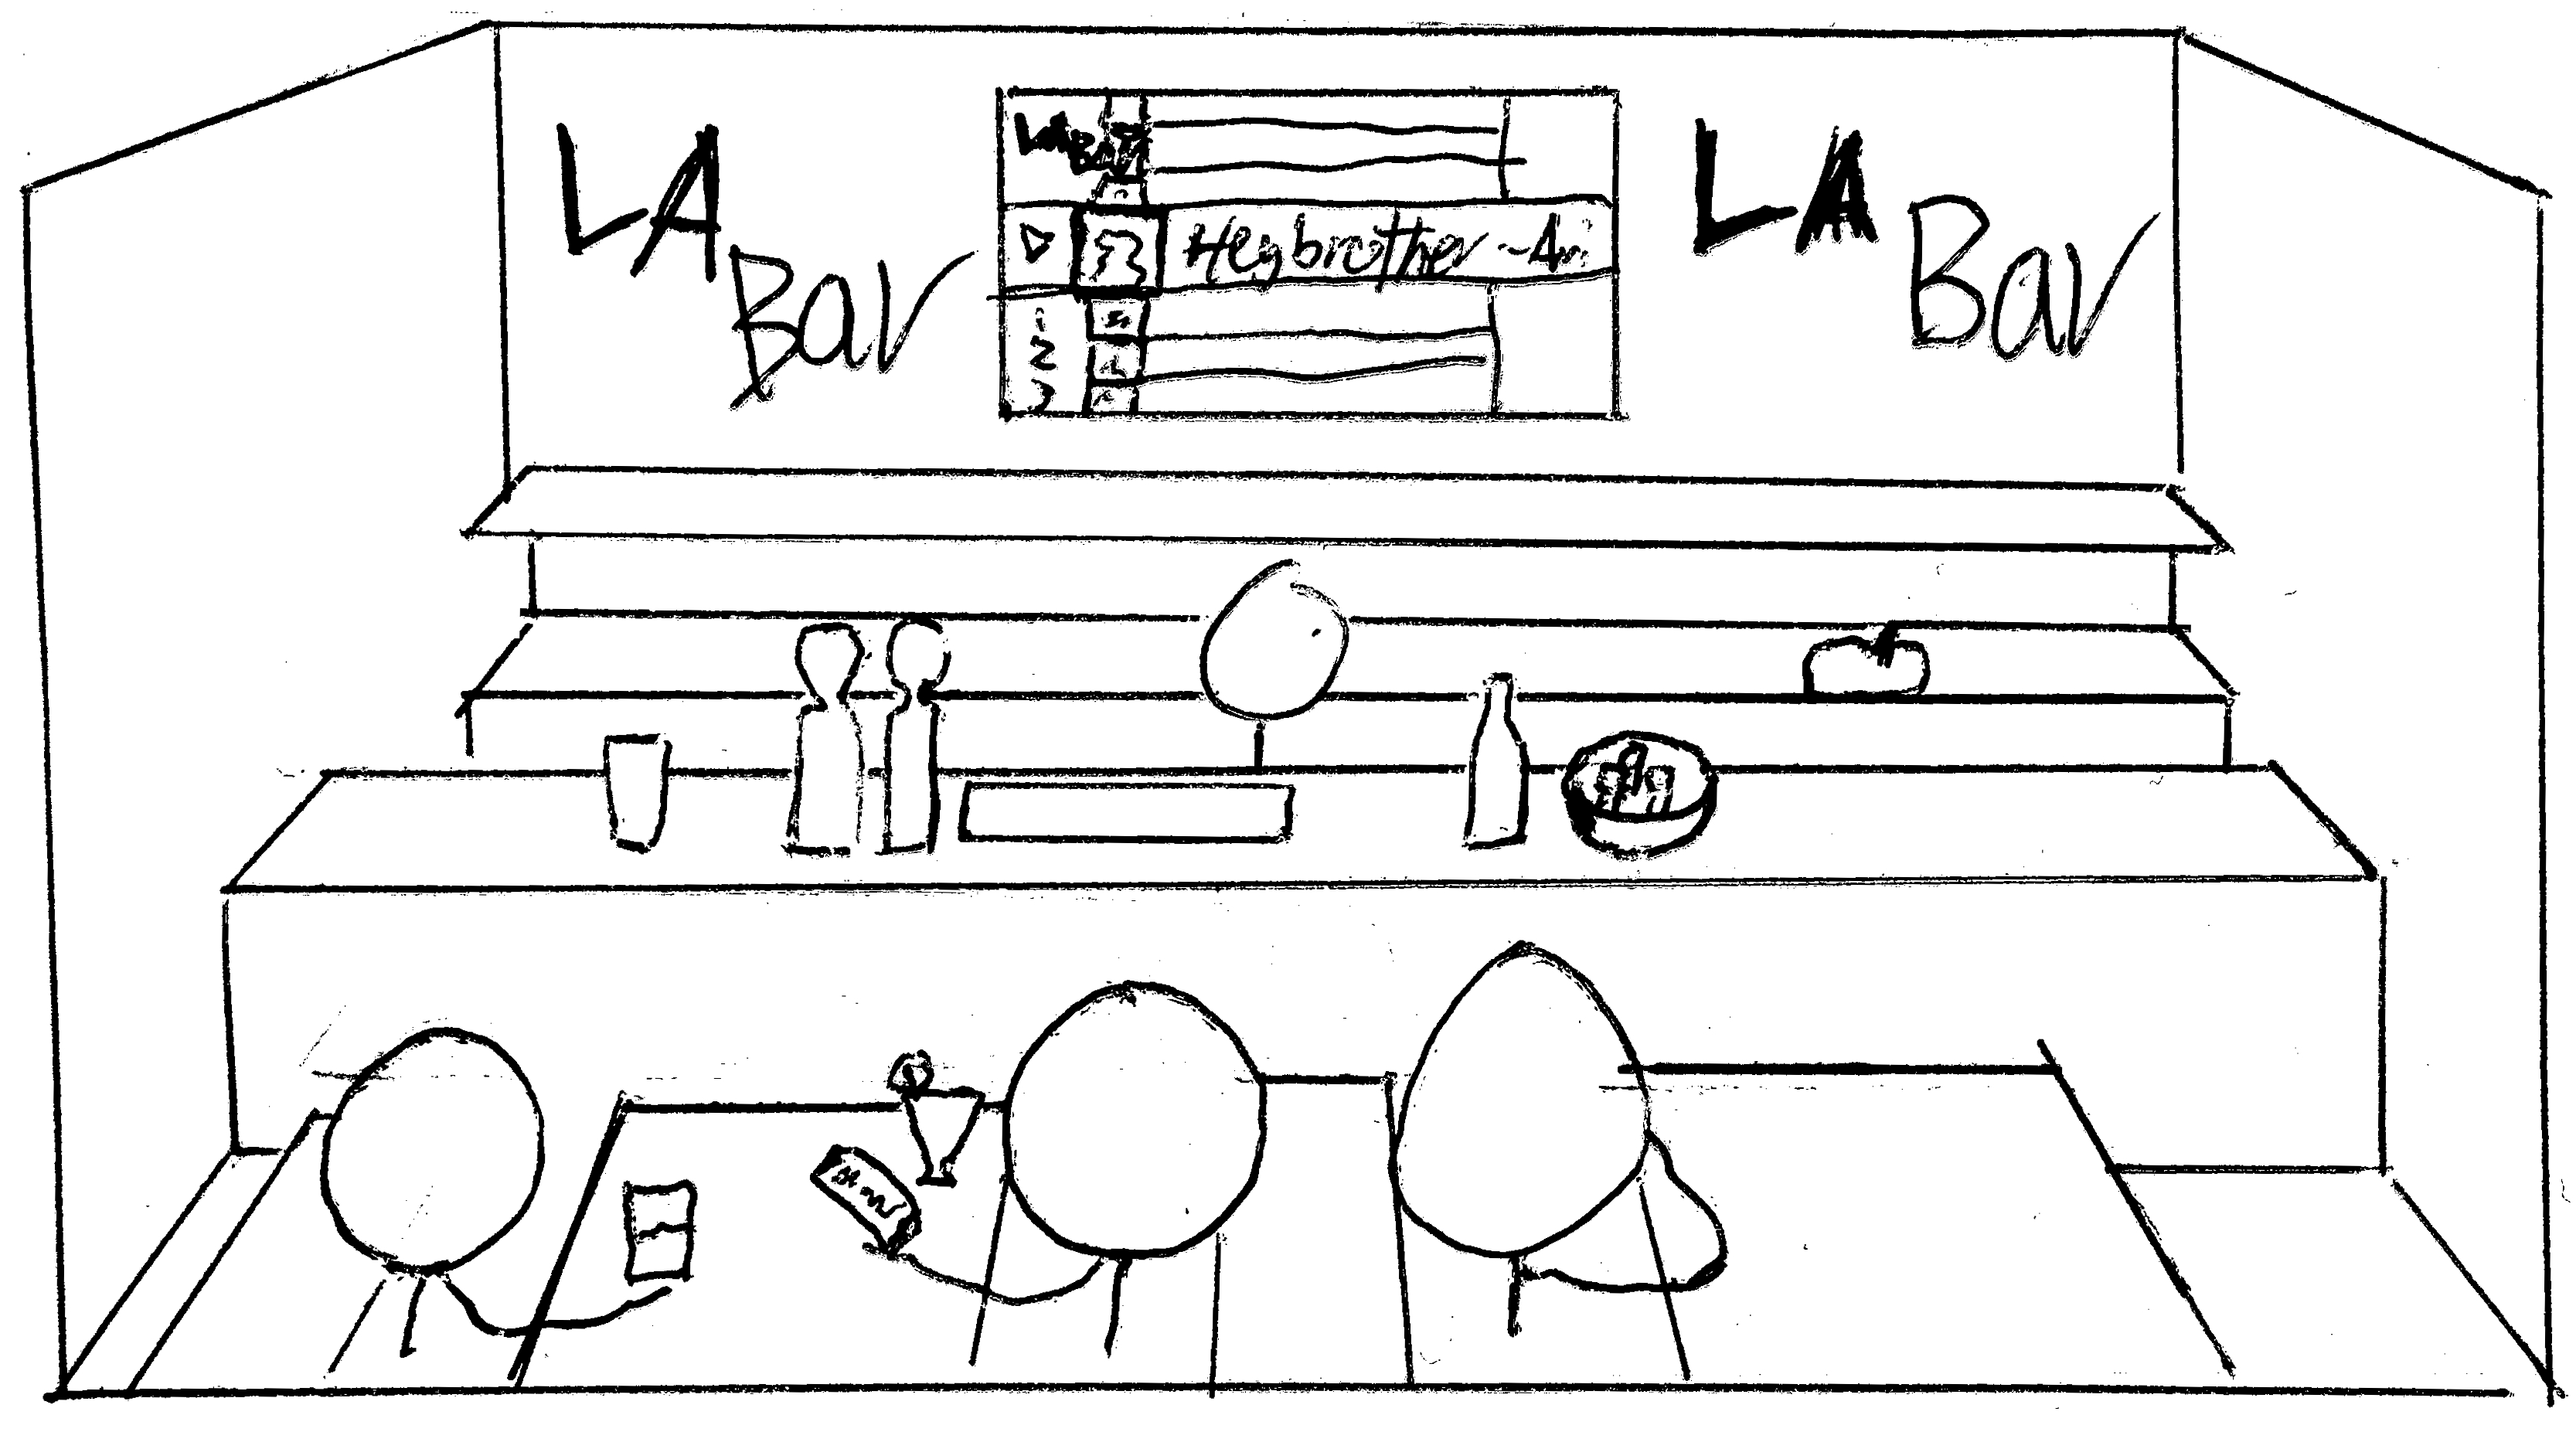
\includegraphics[width=1.0\linewidth]{Images/presentation.png}
  \caption{Sketch of the screen in context and visual design.}\label{fig:PresentationInterface}
\end{figure}

\begin{figure}[hbtp]
  \centering
  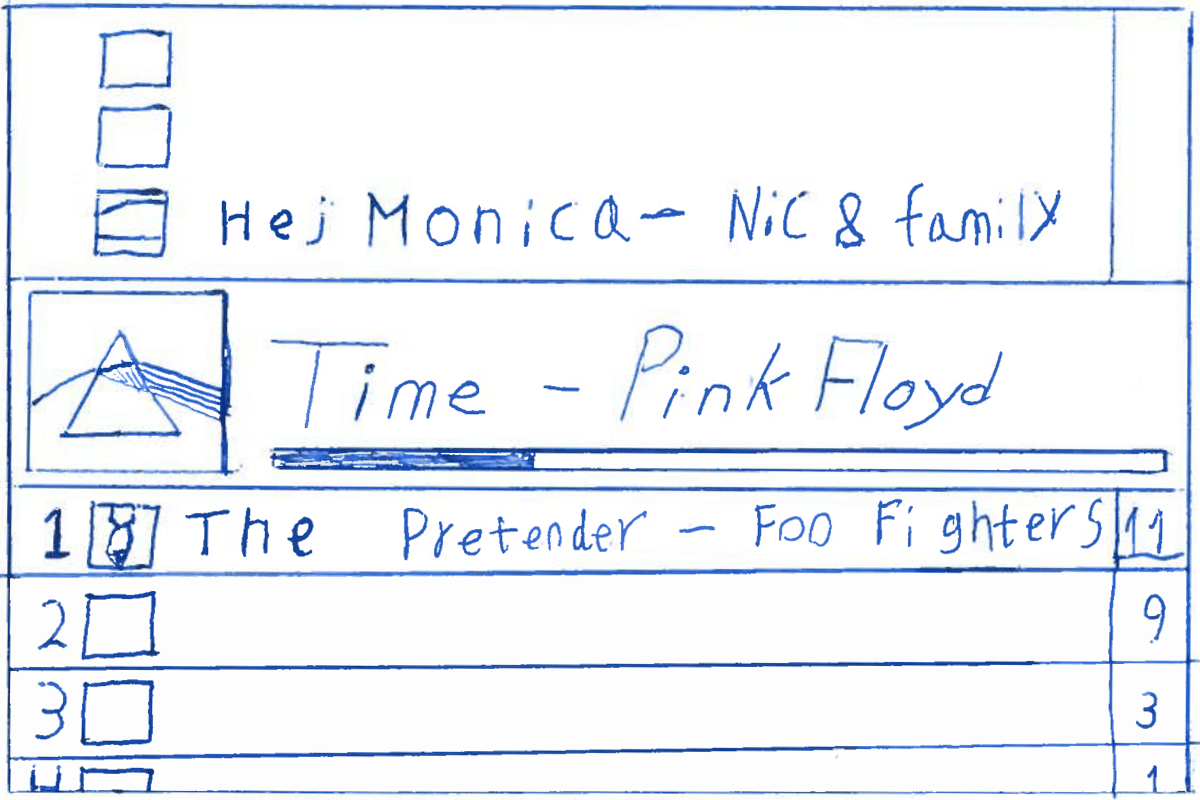
\includegraphics[width=1.0\linewidth]{Images/presentationInterface.png}
  \caption{A sketch of the visual design of the presentation interface.}\label{fig:presentation}
\end{figure}

The idea behind the design of the presentation interface, see \cref{fig:presentation}, is that the user is looking at a screen, that is scrolling the playlist of the venue, where the vertical middle is the currently playing track. The list above is the history of th playlist in accending order from the middle according to number tracks since they were played. Below is the upcoming tracks of the playlist in descending order according number of votes each track has.
